\chapter{精神分裂症的思想和意志障碍} \label{chap:chap60}

在本章和下一章中,我们将研究影响知觉、思想、情绪、情绪和动机的疾病:
精神分裂症、抑郁症、双相情感障碍和焦虑症。
这些一直很难理解,但最近在遗传分析方面的进展已经开始为它们的发病机制提供重要线索。


精神疾病对个人、家庭和社会都有破坏性影响。
世界卫生组织报告说,总体而言,精神疾病构成了全世界残疾的主要原因,并且是世界卫生组织报告的每年 800,000 例自杀的主要风险因素。
此外,抑郁症和焦虑症经常与糖尿病、冠状动脉疾病、中风和其他几种疾病同时发生并恶化其结果。


20 世纪中叶发现的抗精神病药、锂和抗抑郁药等药物使关闭大型且通常不合格的精神病院成为可能;
然而,中途宿舍和其他限制较少的治疗场所并没有足够多地实现。
结果,许多患有精神分裂症和严重双相情感障碍的人在一生中的某个时候变得无家可归,而且在许多国家,患有严重精神障碍的人占监狱人口的很大一部分。


此外,虽然抗精神病药物、锂盐和抗抑郁药物在控制精神障碍症状方面发挥了重要作用,但治疗效果仍然存在很大局限性。
例如,对于高度致残的认知障碍和精神分裂症的缺陷症状没有有效的治疗方法。
即使对于可以从现有药物中获益的症状,如幻觉和妄想,残留症状仍然存在并且复发是常态。
由于人脑带来的重大科学挑战和精神障碍动物模型的局限性,50 多年来精神药物的疗效几乎没有进步。
然而,人类遗传学和神经科学的最新进展为改善这种不幸的状况创造了重要机会。



\section{精神分裂症的特征是认知障碍、缺陷症状和精神病症状}

在医学中,对疾病的理解及其诊断最终基于两个特征的识别:
(1) 病因学因素(例如,微生物、毒素或遗传风险)和 
(2) 发病机制(通过 哪些病原体会导致疾病)。
虽然人类遗传学和神经科学开始深入了解精神分裂症、双相情感障碍和自闭症谱系障碍等疾病的病因和发病机制,但这项研究尚未产生客观的诊断测试或生物标志物。
因此,精神病学诊断仍然依赖于对患者症状的描述、检查者的观察以及随着时间推移的病程。


精神分裂症是一种非常严重的疾病。
其症状可分为三类:
(1)认知症状; 
(2) 缺陷或阴性症状; 
(3) 精神症状。
这些症状群表现出不同的发作时间模式——认知障碍和缺陷症状通常最早出现。
不同的发病时间和每个簇的确切症状被认为是由发育致病机制对不同神经回路和大脑区域的影响造成的。
因此,作用于疾病过程的一个“下游”方面的抗精神病药物等现有治疗方法对认知障碍或缺陷症状没有任何有益影响。


20 世纪初,德国的 Emil Kraepelin 认识到认知能力下降是精神分裂症的一个显着特征,因为精神病症状会出现在多种精神疾病中。
事实上,Kraepelin 对后来被称为精神分裂症的术语是早发性痴呆,这个术语强调了认知丧失的早期发作。
精神分裂症的认知障碍针对工作记忆和执行功能、陈述性记忆、语言流畅性、识别面部表情所传达的情绪的能力以及社会认知的其他方面。
现有药物并不能显着改善这些损伤,但正在进行的研究表明,以认知矫正为目标的心理疗法带来的益处虽然不大,但很有前景。


缺陷症状包括情绪反应迟钝、社交互动退缩、思想和言语内容贫乏以及动力丧失。
精神病症状包括幻觉、妄想和思维紊乱,例如联想松弛(方框 60-1)。
精神分裂症的精神病症状对抗精神病药物有反应。
这些药物还可以减少其他神经精神疾病中出现的精神病症状,包括双相情感障碍、严重抑郁症和神经退行性疾病,如帕金森病、亨廷顿病和阿尔茨海默病。



\subsection{精神分裂症具有在生命的第二个和第三个十年发病的特征性病程}

精神分裂症影响全球 0.25\% 至 0.75\% 的人口,区域差异很小。
男性比女性更容易受到影响,性别比例估计为 3:2,而且男性发病通常较早。
精神分裂症通常开始于青少年后期或二十出头至中期。
持续的认知和缺陷症状通常在精神病症状出现前几个月甚至几年就开始了。
这一时期被一些研究人员称为超高风险状态,而其他人则称为精神分裂症前驱症状。


处于这种风险状态的个人通常会出现可测量的认知功能下降,并伴有社会孤立、多疑以及参与学校工作或其他任务的动力下降等症状。
减轻的精神病性症状通常随之而来,包括短暂的和轻度的幻觉。
并非每个有此类症状的青少年都会发展出所有症状,从而诊断出精神分裂症。
一小部分恢复;
其他人则发展出精神分裂症以外的严重精神疾病。
抗精神病药物似乎不会使处于危险状态的个体受益,也不会延缓精神分裂症的发作。
然而,谈话疗法和通过基于计算机的方法提供的旨在认知矫正的疗法显示出延迟精神病发作的希望。



\subsection{精神分裂症的精神病症状往往是发作性的}

精神症状,包括幻觉和妄想,是精神分裂症最显着的表现。
幻觉是在没有适当的感觉刺激的情况下发生的知觉,它们可能发生在任何感觉方式中。
在精神分裂症中,最常见的幻觉是听觉幻觉。
通常,受影响的人会听到声音,但噪音和音乐也很常见。
有时,这些声音会进行对话,并且经常被视为贬损或欺凌。
偶尔,声音会向受影响的个人发出命令,这可能会对自己或他人造成伤害的高风险。


妄想是没有现实基础的坚定信念,不能用患者的文化来解释,也不能通过论证或证据来改变。
妄想的形式可能千差万别。 对于一些受影响的人来说,现实被严重扭曲:
世界充满了只为受影响的人准备的隐藏迹象(参考想法),或者这个人认为他正在被密切监视、跟踪或迫害(偏执妄想)。
其他人可能会经历奇怪的错觉;
例如,他们可能认为有人正在将思想插入他们的思想或从他们的思想中提取思想,或者他们的近亲已被来自另一个星球的外星人所取代。
除了患者持久的认知障碍外,精神病发作还经常伴有思维紊乱和言语古怪(方框 60-1)。


精神病症状也可能发生在其他神经精神疾病中,例如双相情感障碍、重度(单相)抑郁症、各种神经退行性疾病和药物诱发的状态。
然而,通常可以通过相关症状和发病年龄将这些其他病症与精神分裂症区分开来。
一旦精神分裂症变得完全明显,精神病症状往往是偶发的。
伴有显着紊乱的思维、情绪和行为的严重精神病期穿插于精神病性症状较轻甚至不存在的时期。
精神病发作通常需要住院治疗;
抗精神病药物可显着缩短此类发作的严重程度和持续时间。
第一次和第二次精神病发作通常对抗精神病药物有完全反应,但认知障碍和缺陷症状通常会持续存在。
在最初几次精神病复发后,精神分裂症患者通常会在急性复发之间出现残留的精神病症状,并且尽管接受了抗精神病药物治疗,但仍会出现这些症状。
认知和社会功能通常会在数年内持续恶化,直到达到远低于患者病前功能水平的稳定水平。



\section{精神分裂症的风险受基因的高度影响}

早在 1930 年,德国的 Franz Kalman 就研究了精神分裂症的家族模式,并得出结论认为基因起着重要作用。
为了更清楚地将遗传影响与环境影响区分开来,Seymour Kety、David Rosenthal 和 Paul Wender 在丹麦对出生时或出生后不久被收养的儿童进行了检查。
他们发现,与收养家庭的精神分裂症发病率相比,被收养人的生物学家庭中的精神分裂症发病率更能预测精神分裂症。


Kety 和他的同事还观察到,一些患有精神分裂症的被收养人的生物学亲属表现出与精神分裂症相关的较轻的症状,例如社会孤立、多疑、古怪的信念和神奇的思维,但不是坦率的幻觉或妄想。
自 Kety 时代以来,人们观察到这些亲属也可能表现出介于未受影响个体和精神分裂症患者之间的认知障碍。
他们还可能表现出通过磁共振成像观察到的大脑皮层变薄,这也介于健康个体和精神分裂症患者之间。 
(精神分裂症的皮层变薄将在下文讨论。)
这些人现在被诊断出患有精神分裂症,这似乎是精神分裂症谱系中较温和的一端。
症状的严重程度和性质似乎受到个人风险相关遗传变异的总体负担以及暴露于环境风险因素的影响。


欧文·戈特斯曼 (Irving Gottesman) 对丹麦精神分裂症患者扩展系谱的研究支持了基因的重要性。
Gottesman 注意到亲属患精神分裂症的风险与他们与受影响的人共享 DNA 序列的程度之间的相关性。
他发现一级亲属(包括父母、兄弟姐妹和孩子,他们与患者有 50\% 的 DNA 序列)比二级亲属(包括阿姨、叔叔、侄女、侄子和孙辈)患精神分裂症的终生风险更高, 他们共享 25\% 的 DNA 序列)。
即使是三级亲属(仅共享患者 12.5\% 的 DNA 序列)患精神分裂症的风险也高于一般人群中约 1\% 的患此病风险(图 \ref{fig:60_1})。


\begin{figure}[htbp]
	\centering
	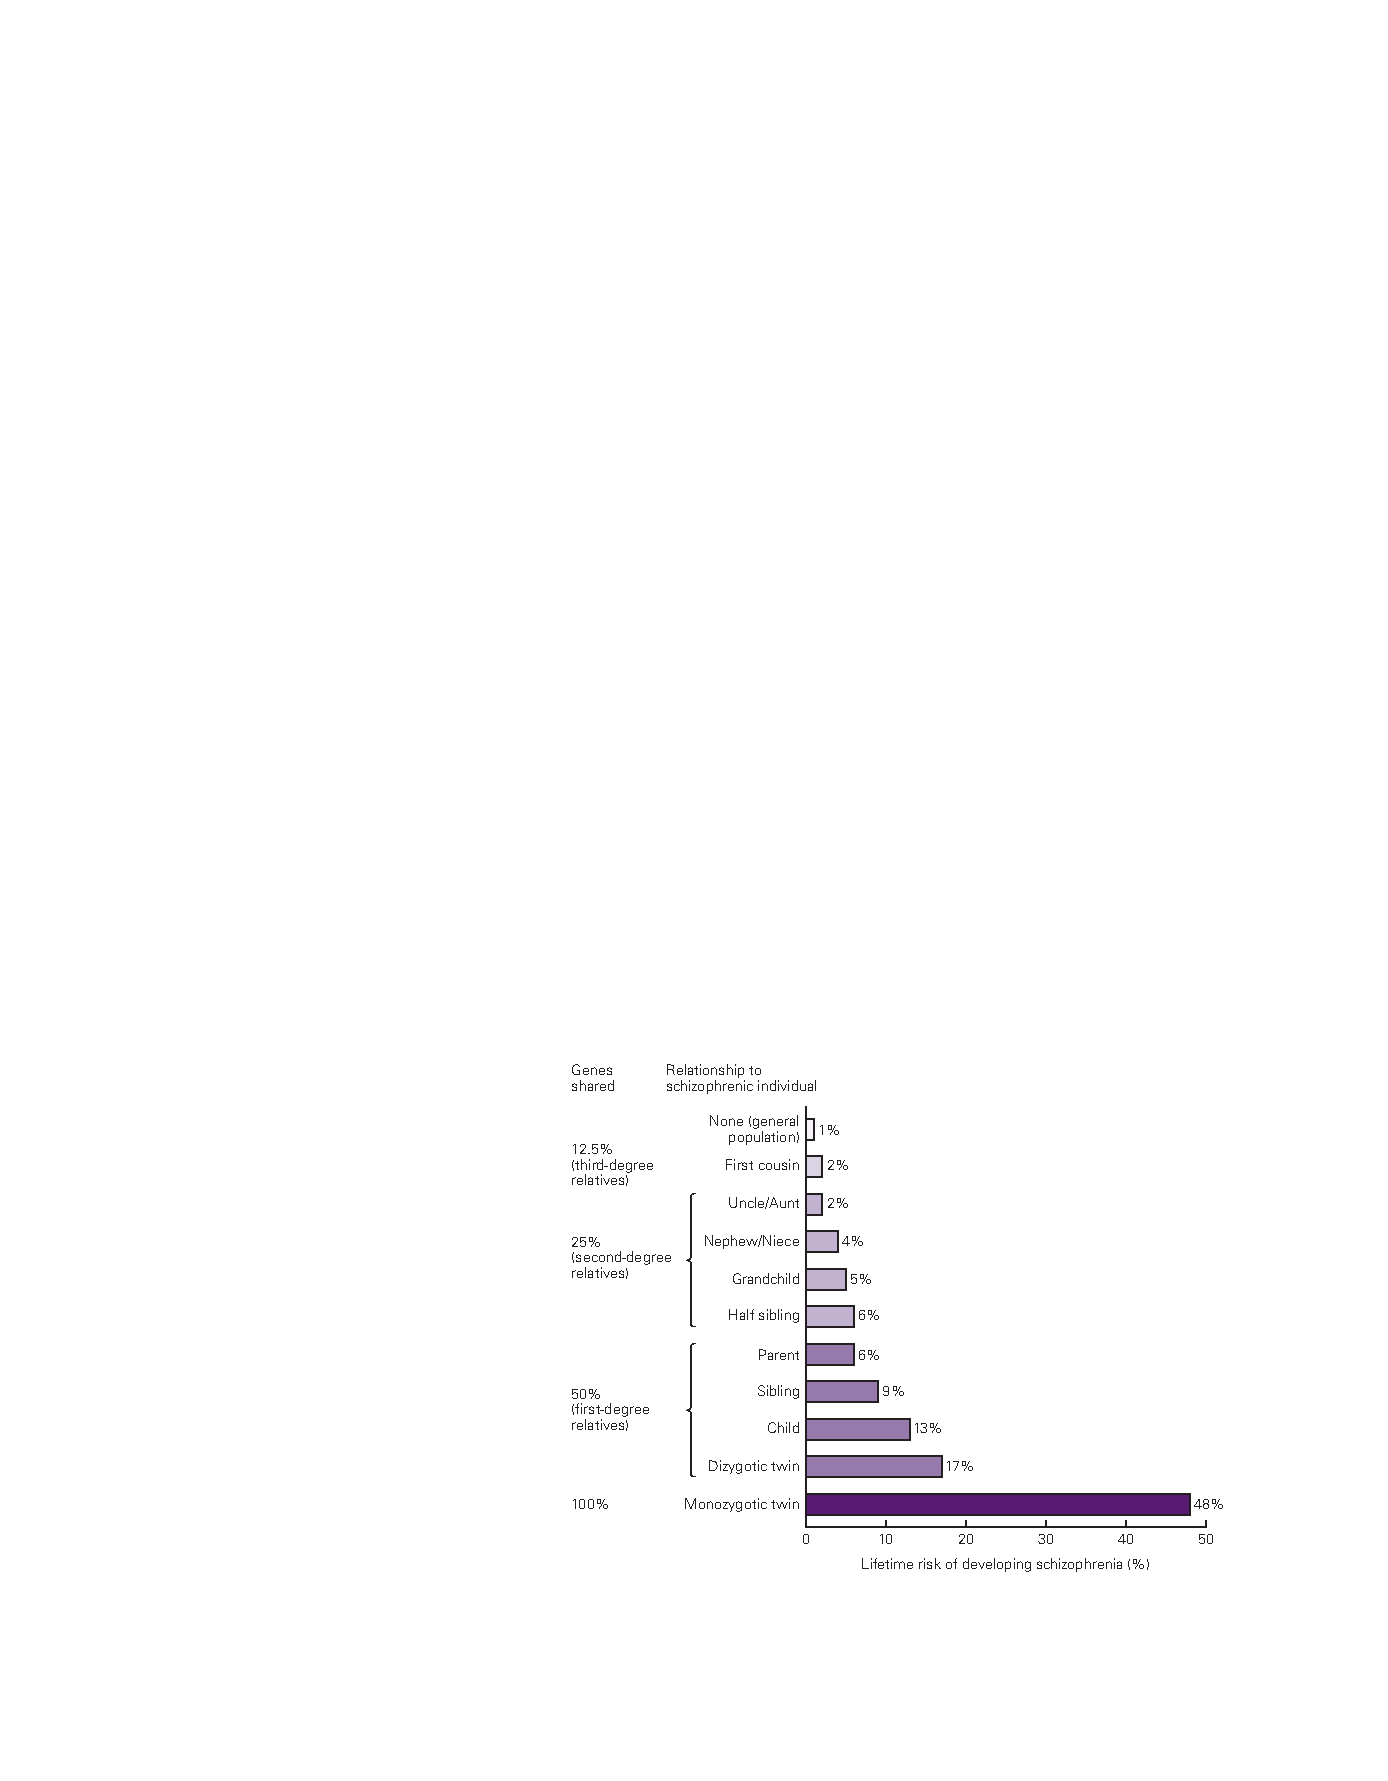
\includegraphics[width=0.7\linewidth]{chap60/fig_60_1}
	\caption{精神分裂症的终生风险随着与精神分裂症患者的遗传相关性而增加。 精神分裂症的风险随着受影响个体的遗传相关性而增加,因此,随着 DNA 序列共享的增加。 然而,家庭隔离模式并不遵循简单的孟德尔比率; 相反,遗传反映了基因的复杂性。 此外,风险在相关性类别(一级和二级亲属)内有所不同,表明未共享的发展或环境影响的作用。 (经许可转载自 Gottesman 1991。)}
	\label{fig:60_1}
\end{figure}


根据 Gottesman 在这些谱系中测得的风险水平差异,他认识到精神分裂症风险不会像孟德尔显性或隐性特征那样在家族内传播(即,它不是由单一基因位点引起的)。
他正确地预测,精神分裂症是一种多基因特征,涉及整个人类基因组中的大量位点。
这种遗传结构是许多人类表型(包括疾病表型)的基础,并且可能涉及基因组中的数百个位点。
在多基因性状中,每个与疾病相关的位点的变异对表型的贡献很小,且具有累加效应。
遗传风险变异与环境因素共同作用产生精神分裂症表型。


2014 年,一个大型全球财团报告了一项针对超过 35,000 名精神分裂症患者的全基因组关联研究。
该研究确定了 108 个与精神分裂症相关的全基因组重要位点,这些位点分布在整个基因组中。
研究仍在继续,已知基因座的数量已经超过 250 个。
这些基因座中的每一个都代表一个由单核苷酸多态性识别的 DNA 片段,它赋予精神分裂症风险的小幅增加(通常为 5\%–10\%)。
这种等位基因变异的价值在于作为一种工具来识别在疾病分子机制中起作用的基因。
反过来,相关基因有助于识别可能在治疗药物开发中被利用的分子途径。


除了利用遗传学发现与疾病有关的生物学过程外,它还有助于在流行病学和临床研究中对研究人群进行分层。
一个人患精神分裂症或其他疾病的风险可以通过计算他或她对该病症的常见风险等位基因的总负担来估计。
结果是多基因风险评分,该指标越来越多地用于在临床研究和环境风险因素的流行病学研究中根据对精神分裂症的遗传易感性对人群进行分层。


跨研究重复的精神分裂症的环境风险因素包括子宫内营养缺乏(特别是在饥荒后的研究中)、出生季节(冬季和早春出生)、城市出生和迁移。
在如此广泛的暴露类别中分析致病因素可能会受益于了解谁是易感者。
此外,环境诱发因果途径的线索可以在具有特定暴露的精神分裂症患者的风险基因型中找到。


由于缺乏客观的诊断测试,目前的诊断标准,例如第五版《精神疾病诊断和统计手册》中的标准,都是基于临床观察和病程。
因此,目前被诊断患有精神分裂症的个体存在高度异质性。
多基因风险评分只能解释精神分裂症队列中的部分差异,并且评分仅提供概率信息。
然而,它们代表了第一个允许对诊断为精神分裂症的受试者进行分层的客观工具。
因此,此类评分的应用可能会开始减少从神经影像学到神经生理学研究再到治疗试验的临床研究中的异质性。


尽管几乎所有精神分裂症病例都反映出多基因风险,正如 Gottesman 预测的那样,但一小部分病例受到渗透突变的高度影响,这种突变通常会产生多效性影响,包括智力障碍,导致通常称为综合征型精神分裂症。
这些渗透突变中的大多数是拷贝数变异:染色体特定片段的缺失、重复或有时三次重复。


综合征型精神分裂症最常见和研究最充分的原因是 22q11.2 微缺失,约占诊断为精神分裂症患者的 1\%。
微缺失通常从头发生并导致 38 至 44 个基因的两个拷贝之一丢失。
作为典型的此类拷贝数变异,受影响的人会出现复杂的症状。
伴随 22q11.2 微缺失的综合征,有时称为腭心面综合征或 DiGeorge 综合征,包括认知障碍、心血管缺陷和面部畸形。
这些症状和体征中每一个的外显率都独立于其他症状和体征;
因此,受影响的个体具有不同的表型组合。
具有 22q.11.2 微缺失的个体患精神分裂症的风险为 25\% 至 40\%,患自闭症的风险为 20\%。
其他综合征形式的精神病也有类似的变化。


精神分裂症的综合征形式可以为精神病生物学提供重要的窗口,即使它们与常见的多基因类型精神分裂症的相似性仍然是一个研究问题。
渗透突变的一个强大优势是能够生成细胞和动物模型,以表征它们对大脑结构和功能的影响。
第二个优势是能够前瞻性地研究携带这些突变的个体。
因此,研究综合征型精神分裂症有可能揭示很多基本的病理生理机制。
一个重要的研究领域是导致精神病的拷贝数变异和其他高外显率突变如何根据一个人的遗传背景表现出来,特别是许多影响风险的常见 DNA 变异。
就这一点而言,最近的研究结果表明,携带拷贝数变异的个体出现精神病症状的倾向可能是由于拷贝数变异与该人的精神分裂症多基因背景风险之间的强烈相互作用,表明与单一基因相关的精神分裂症之间存在重要的共享机制。 基因突变,并且仅与多基因变异有关。



\section{精神分裂症的特点是大脑结构和功能异常}

通过死后检查和活体患者的各种非侵入性技术,已经在精神分裂症中发现了大脑结构和功能的异常。
通过尸检研究和结构 MRI,最好的重复发现是大脑皮层前额叶、颞叶和顶叶区域的灰质丢失(图\ref{fig:60_2}),同时脑室大小的平衡增加(图 \ref{fig:60_3})。
大脑皮层变薄在背外侧前额叶皮层最为明显,这是一个对工作记忆至关重要的大脑区域,因此对思想、情绪和行为的认知控制至关重要。



\begin{figure}[htbp]
	\centering
	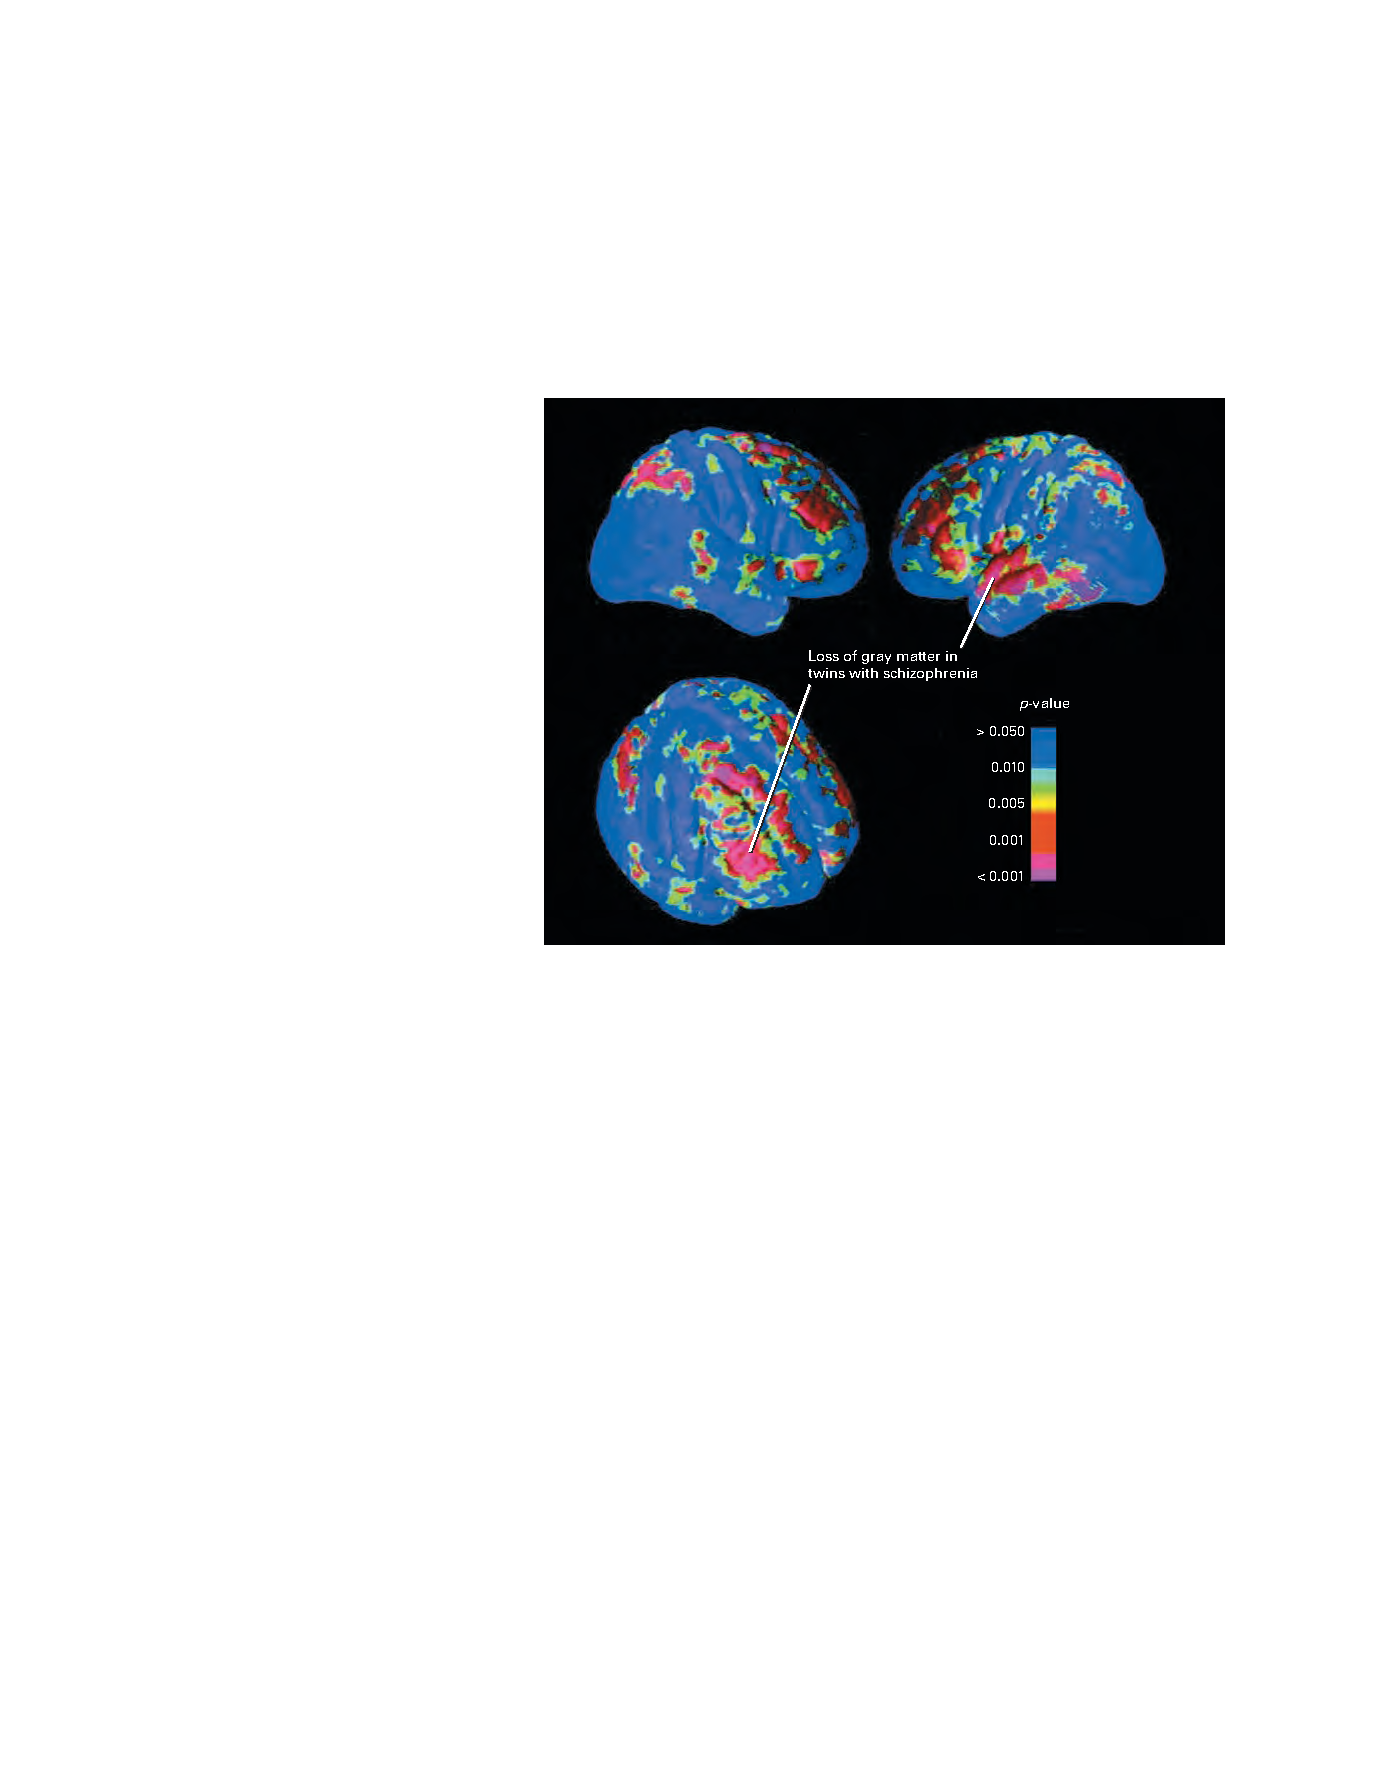
\includegraphics[width=0.7\linewidth]{chap60/fig_60_2}
	\caption{精神分裂症中的灰质丢失。 灰质损失在精神分裂症中有很好的记录。 没有被诊断为精神分裂症的一级亲属仍然经常表现出介于健康个体和被诊断患有精神分裂症的人之间的皮质灰质损失。 与此相一致的是,一项研究检查了与健康匹配的对照双胞胎相比,精神分裂症不一致的同卵双胞胎和异卵双胞胎的皮质灰质损失,发现那些有精神分裂症遗传风险但没有患精神分裂症的人有显着损失。 被诊断患有精神分裂症的双胞胎成员在背外侧前额叶、颞上部和顶叶上部联合区域表现出额外的、疾病特异性的皮质变薄。 这些额外的缺陷似乎反映了参与发病机制的非遗传因素(例如,发育或环境因素)的影响。 疾病特异性灰质损失与认知障碍的程度相关,而不是与疾病持续时间或药物治疗相关。 此处的图像显示了从右侧、左侧和右侧倾斜角度观察的精神分裂症同卵双胞胎相对于健康双胞胎(n = 10 对)的灰质区域缺陷。 双胞胎的差异通过叠加在皮质表面图上的伪彩色标度来说明,粉色和红色表示最大的统计显着性。 (经许可转载自 Cannon 等人,2002 年。)}
	\label{fig:60_2}
\end{figure}


\begin{figure}[htbp]
	\centering
	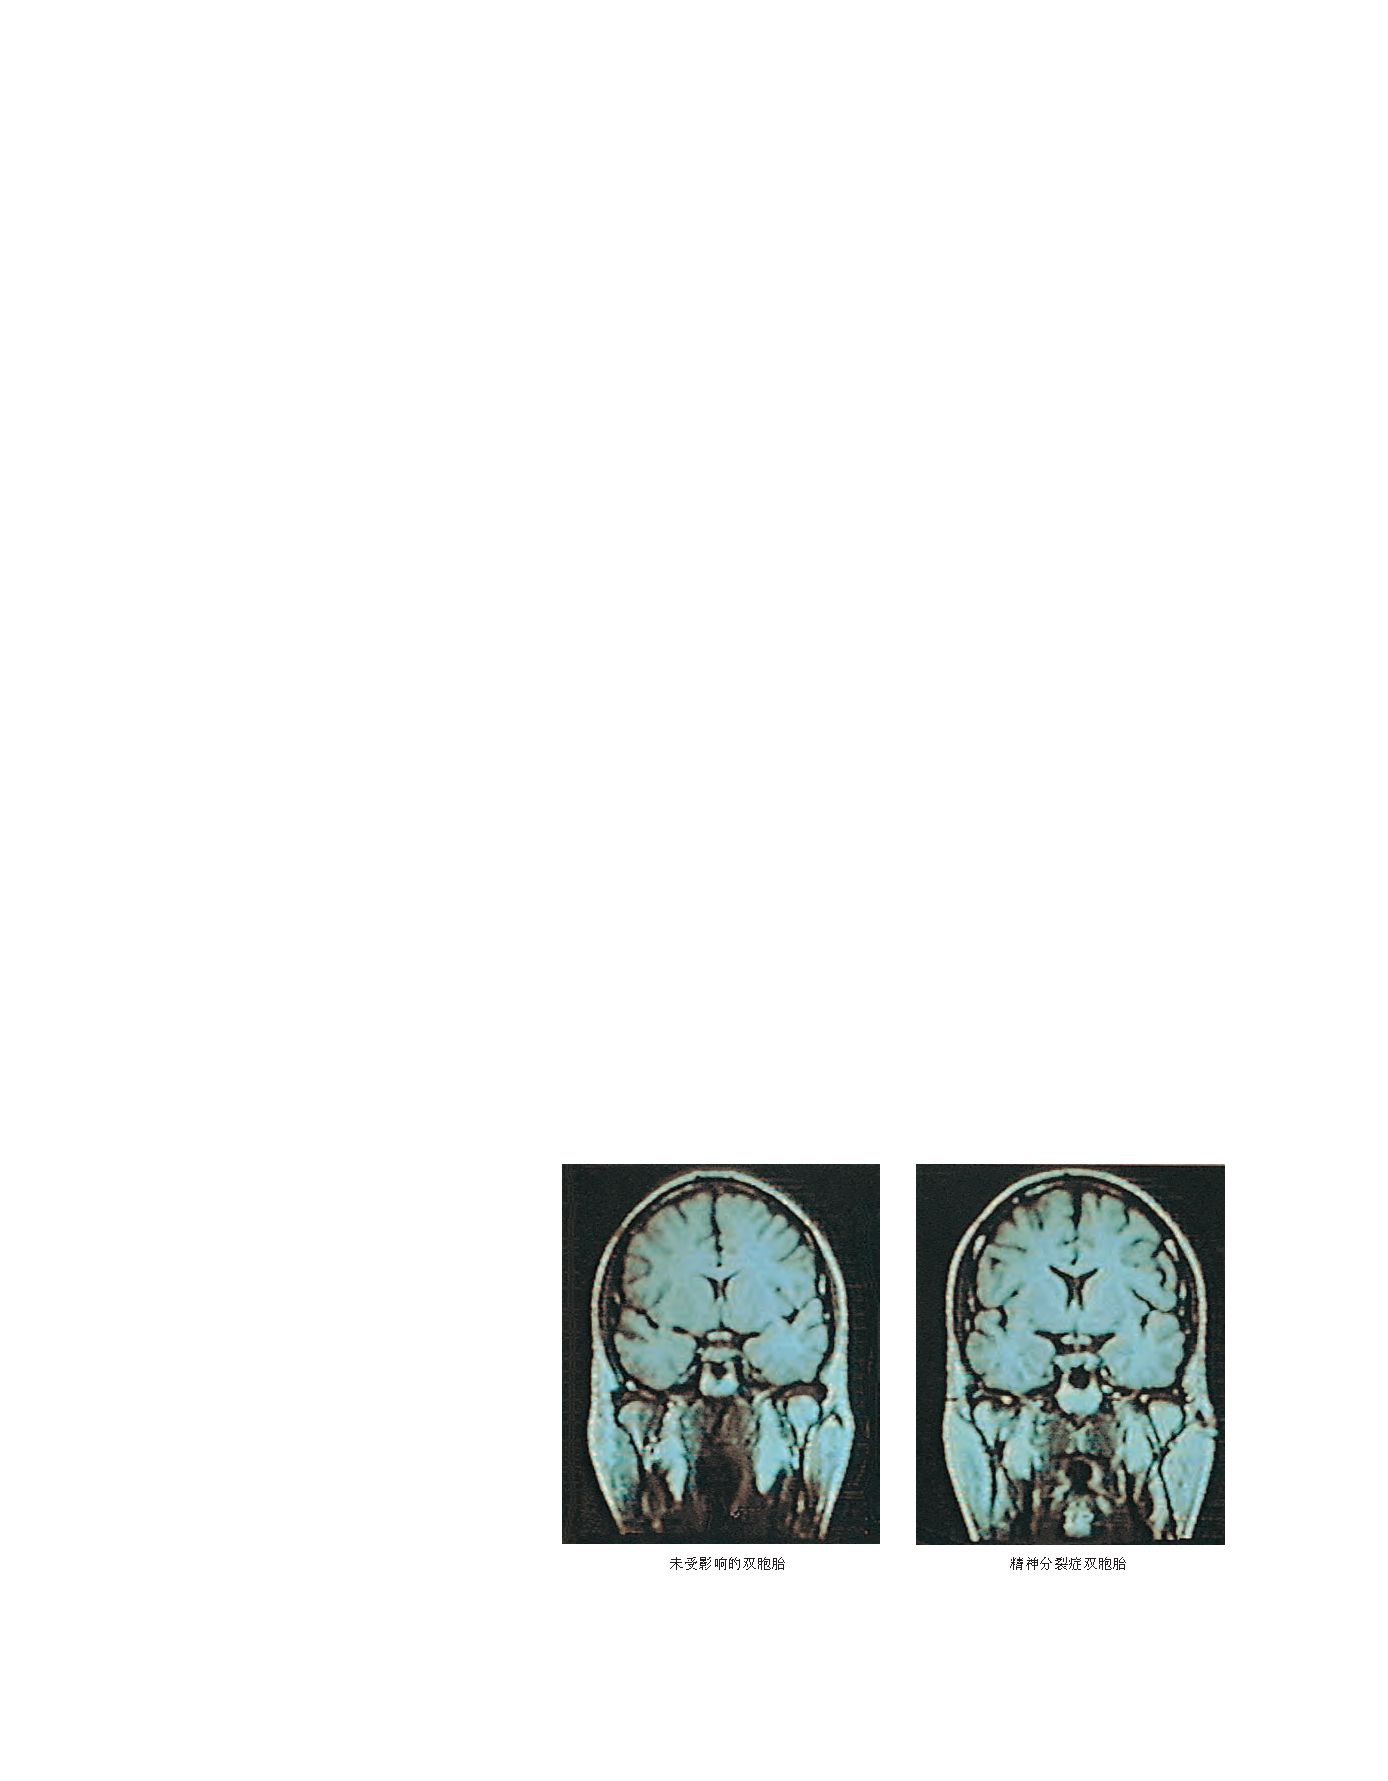
\includegraphics[width=0.7\linewidth]{chap60/fig_60_3}
	\caption{}
	\label{fig:60_3}
\end{figure}


精神分裂症患者颞上回、颞极、杏仁核和海马体中灰质的丢失也与认知障碍、对他人情绪的识别以及受影响者的情绪调节有关。
使用正电子发射断层扫描和功能性 MRI (fMRI) 的功能性神经成像表明,患者在成像时执行工作记忆任务的缺陷与背外侧前额叶皮层激活的减少有关,这是一个已知在工作记忆中起关键作用的大脑区域 (图 \ref{fig:60_4})。


\begin{figure}[htbp]
	\centering
	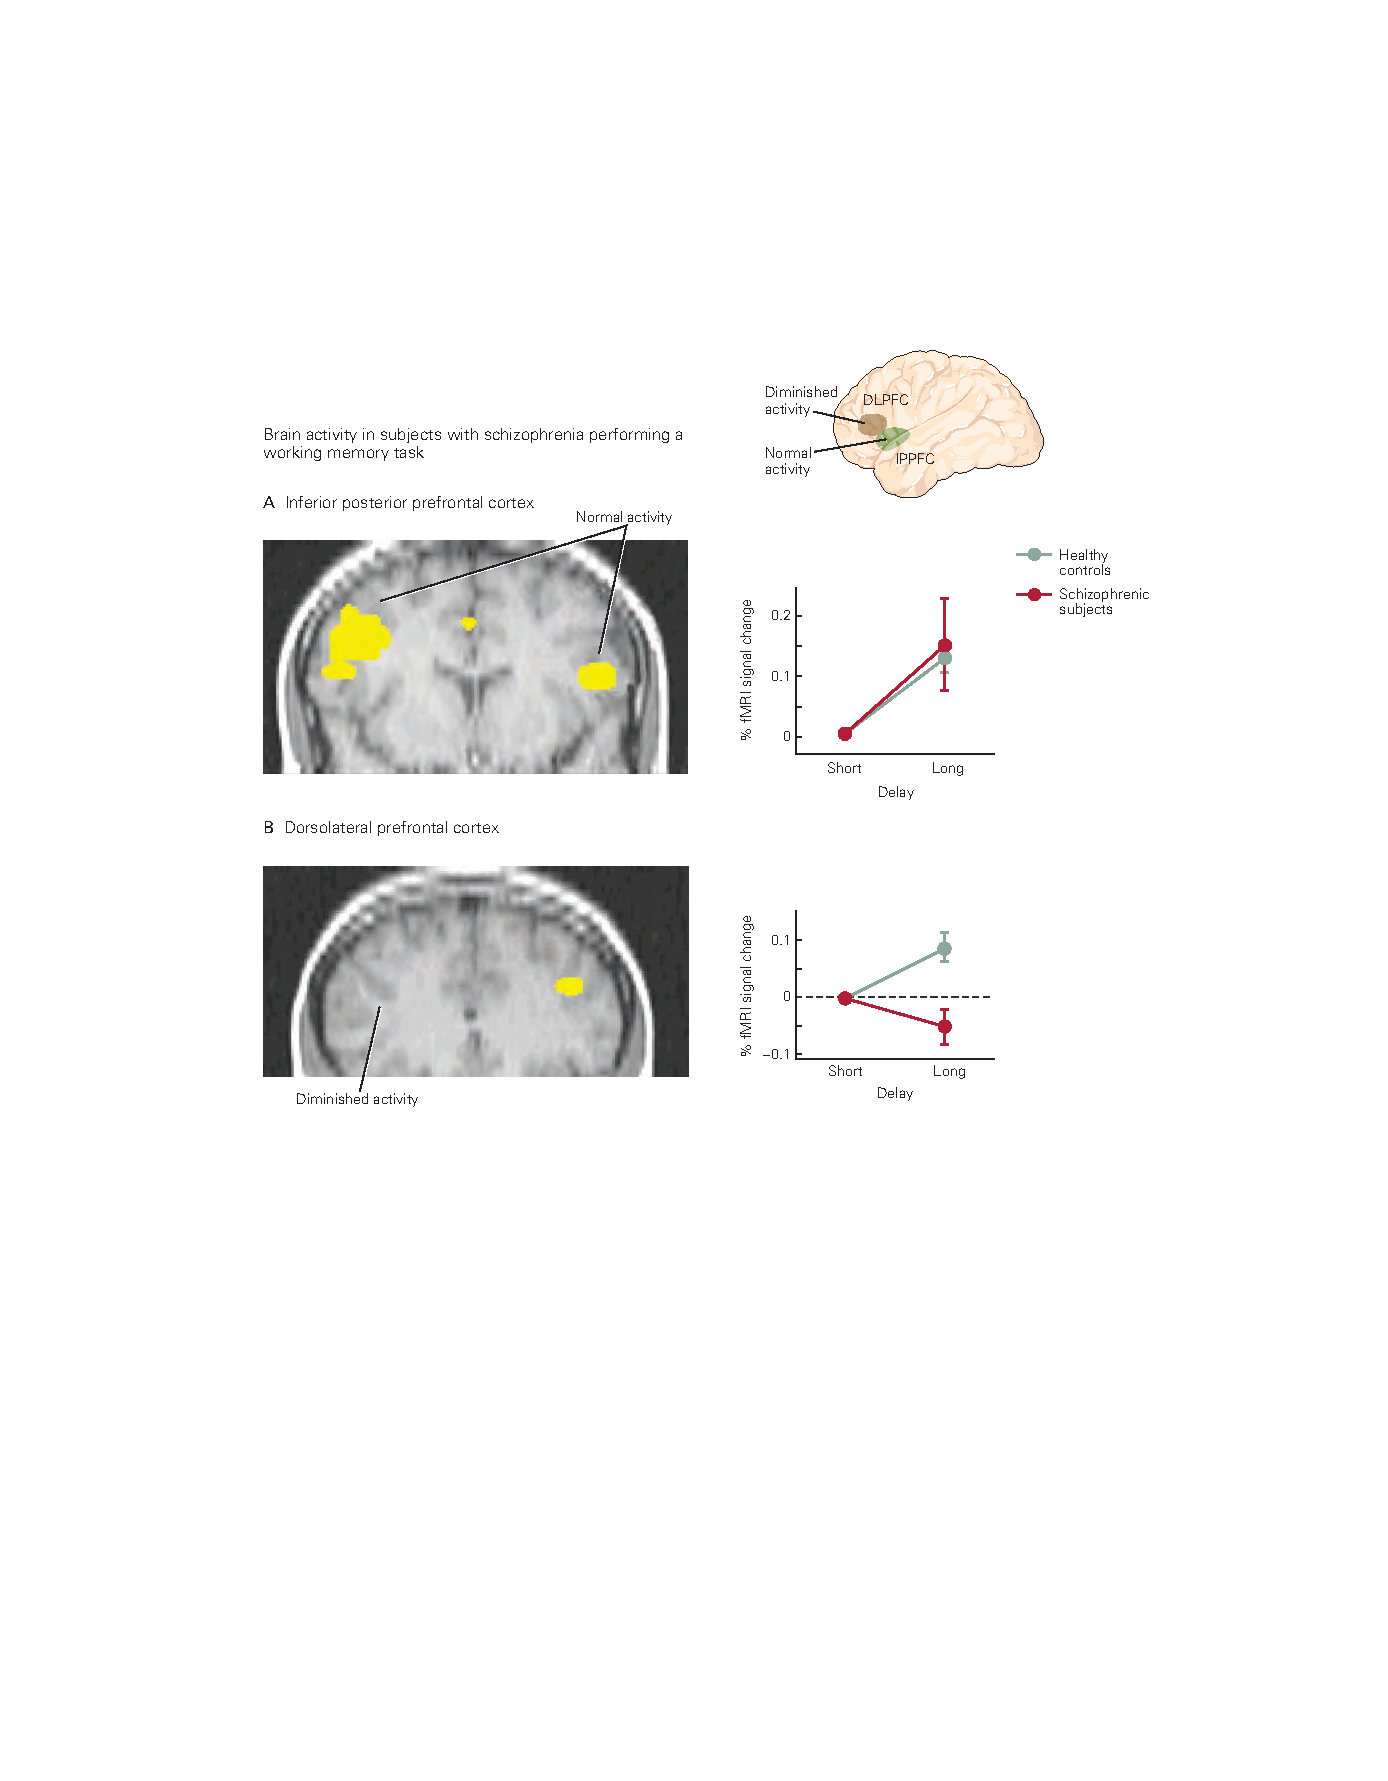
\includegraphics[width=0.8\linewidth]{chap60/fig_60_4}
	\caption{精神分裂症前额叶皮层功能缺陷。 功能性磁共振成像 (fMRI) 用于检验以下假设:精神分裂症患者的工作记忆在前额叶皮层中的回路与对照组不同。 在受试者执行工作记忆任务时,检查了两组患者(精神分裂症患者(从未服用过抗精神病药物的首发患者)和健康对照组)前额叶皮层的活动。 向受试者展示一系列字母,并指示仅当特定字母(“探查”字母)紧跟在另一个特定字母(“上下文提示”字母)之后时,才对特定字母(“探测”字母)做出回应。 通过增加提示和探测字母之间的延迟,增加了对工作记忆的要求。 对工作记忆的更大需求需要更多激活前额皮质电路。 (经许可改编自 Barch 等人,2001 年) 工作记忆表明这些区域的功能在精神分裂症患者中保持完好。 该图显示了健康对照者和精神分裂症患者在长延迟和短延迟条件下前额叶皮层右侧发生的 fMRI 信号变化。 左侧观察到类似的效果。 B. 与健康对照组相比,精神分裂症患者的布罗德曼区 46/49(背外侧前额叶皮层 (DLPFC) 区域)的活动较少。 与 Brodmann 区 44/49(显示在 A 部分)不同,Brodmann 区 46/49 在精神分裂症患者中没有正常激活,这与精神分裂症患者的工作记忆缺陷一致。 前额叶皮层的一个区域与其他似乎具有正常功能的区域的选择性损伤表明该损伤是由于区域特定过程而不是弥漫性和非特异性病理过程。}
	\label{fig:60_4}
\end{figure}


人们也越来越认识到,精神分裂症的特征是大脑区域之间的连接中断(图 \ref{fig:60_5})。
解剖连通性可以通过弥散张量成像来测量,它可以识别大脑区域之间的主要轴突束。
大脑区域之间的功能连通性可以通过测量不同大脑区域的活动模式相互关联的程度来生理估计,使用诸如静息状态 功能性核磁共振和电生理学等方法。
影像学和生理学方法都表明,患有精神分裂症的人大脑区域之间的连接存在缺陷。
较弱的联系可能会损害认知和复杂的行为。


\begin{figure}[htbp]
	\centering
	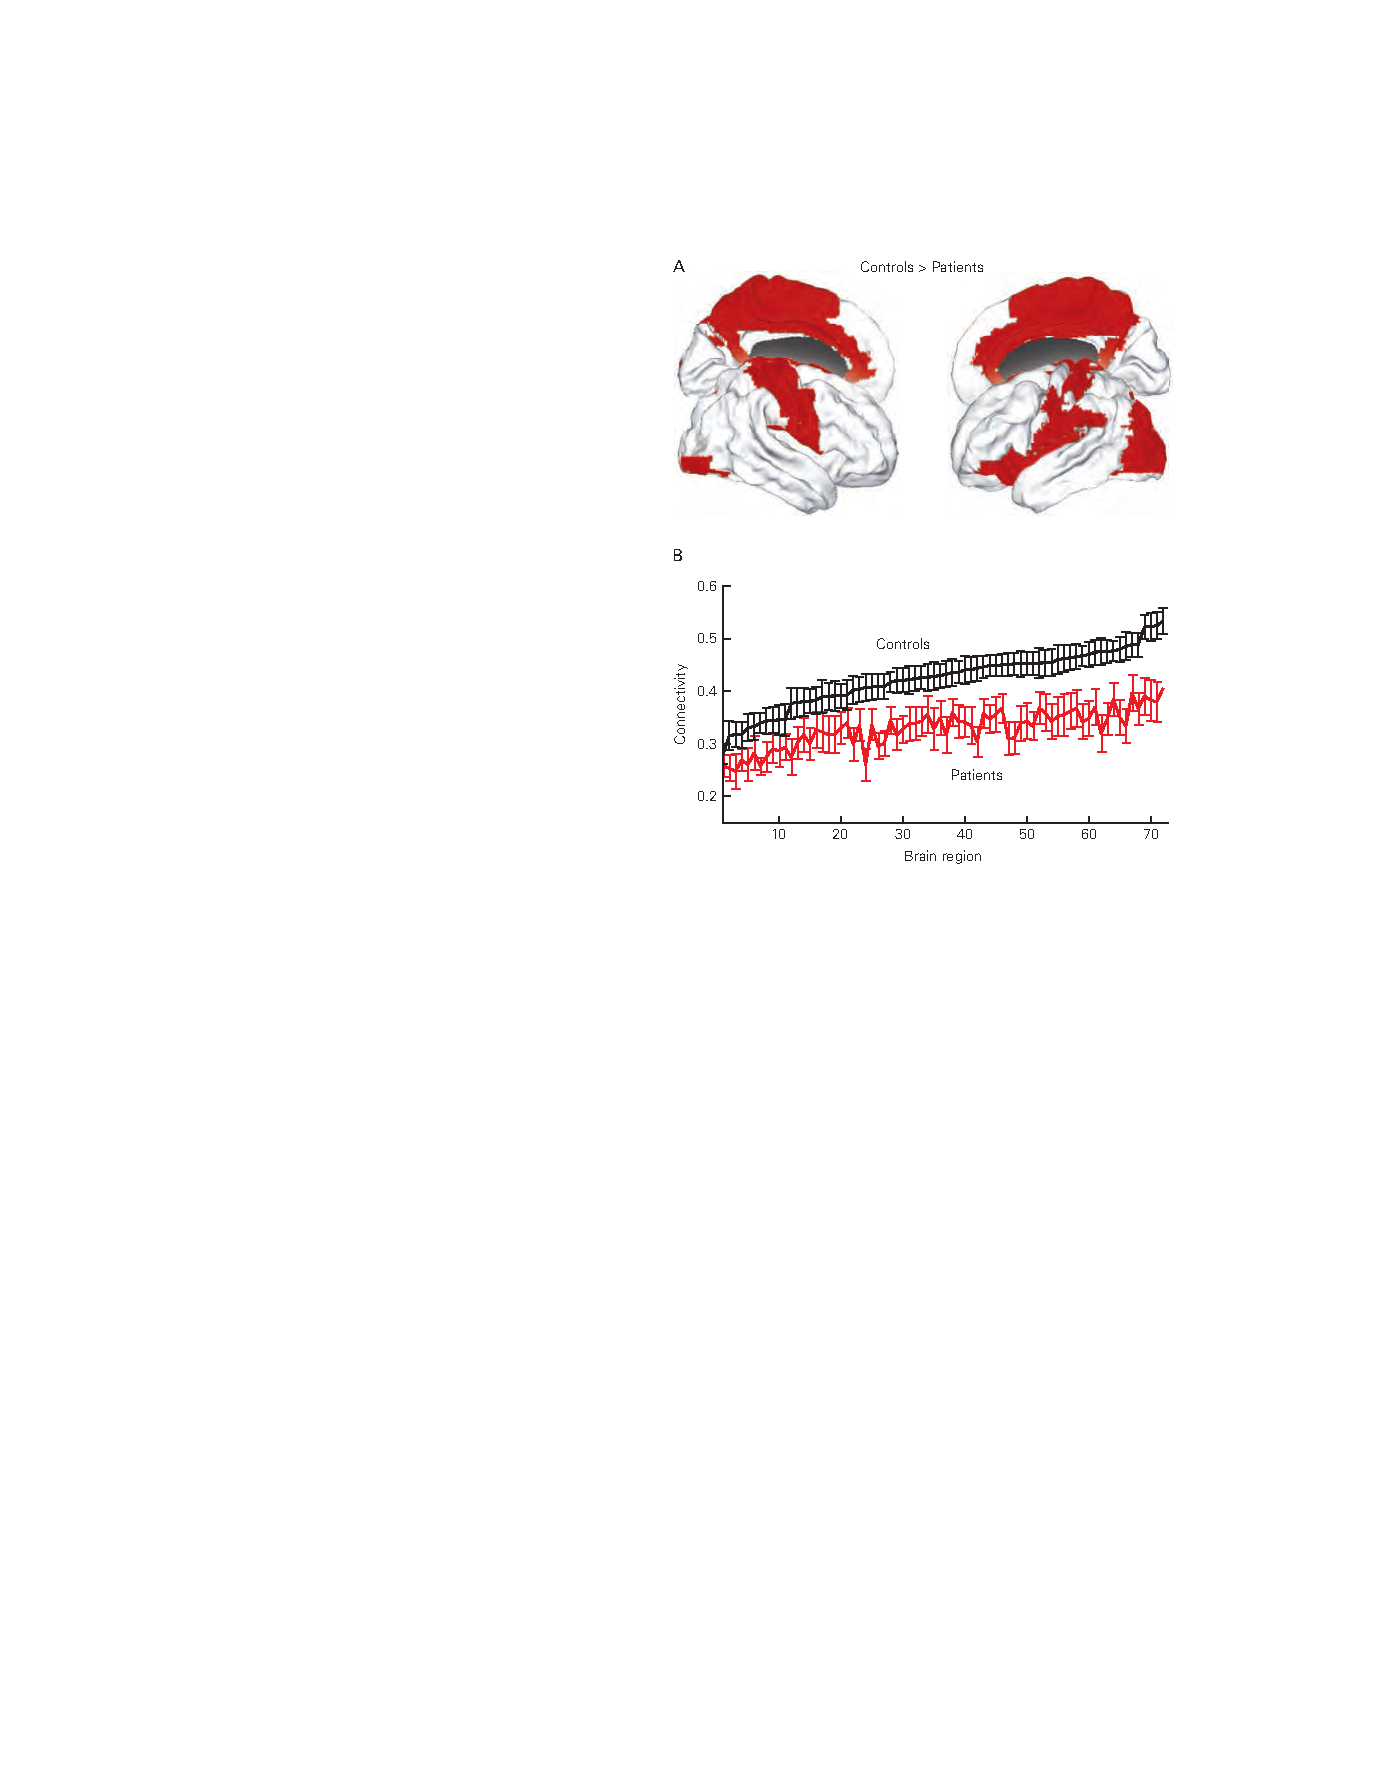
\includegraphics[width=0.6\linewidth]{chap60/fig_60_5}
	\caption{精神分裂症患者的功能连接性下降。 通过静息状态功能磁共振成像测量精神分裂症患者和对照受试者中 72 个确定的大脑区域之间神经活动的相关性。 (经许可转载自 Lynall 等人,2010 年。)A. 与对照组相比,患者功能连接性显着降低的大脑区域以红色突出显示。 B. 患者和健康对照的每个大脑区域和大脑其余部分之间的平均(+/- 平均标准误差)功能连接。}
	\label{fig:60_5}
\end{figure}

\subsection{大脑皮层中灰质的丢失似乎是由突触联系的丢失而不是细胞的丢失引起的}
尸检研究检查了构成精神分裂症大体解剖学发现和功能缺陷基础的细胞异常。 这些研究表明,前额叶和颞叶皮质区域的灰质丢失不是细胞死亡的结果,而是树突状突起减少的结果。 结果,大脑皮层中细胞的堆积密度增加。 每单位体积更多的细胞和更少的总灰质有助于脑室空间的扩大。

锥体神经元(新皮层中最常见的兴奋性神经元类型)上树突和树突棘的减少(图 \ref{fig:60_6})可能意味着精神分裂症患者受影响大脑区域的突触接触缺失。 突触连接的丢失可能是远程功能连接异常以及在需要工作记忆的任务中无法募集前额皮质区域的原因(图 \ref{fig:60_4} 和 \ref{fig:60_5})。

\begin{figure}[htbp]
	\centering
	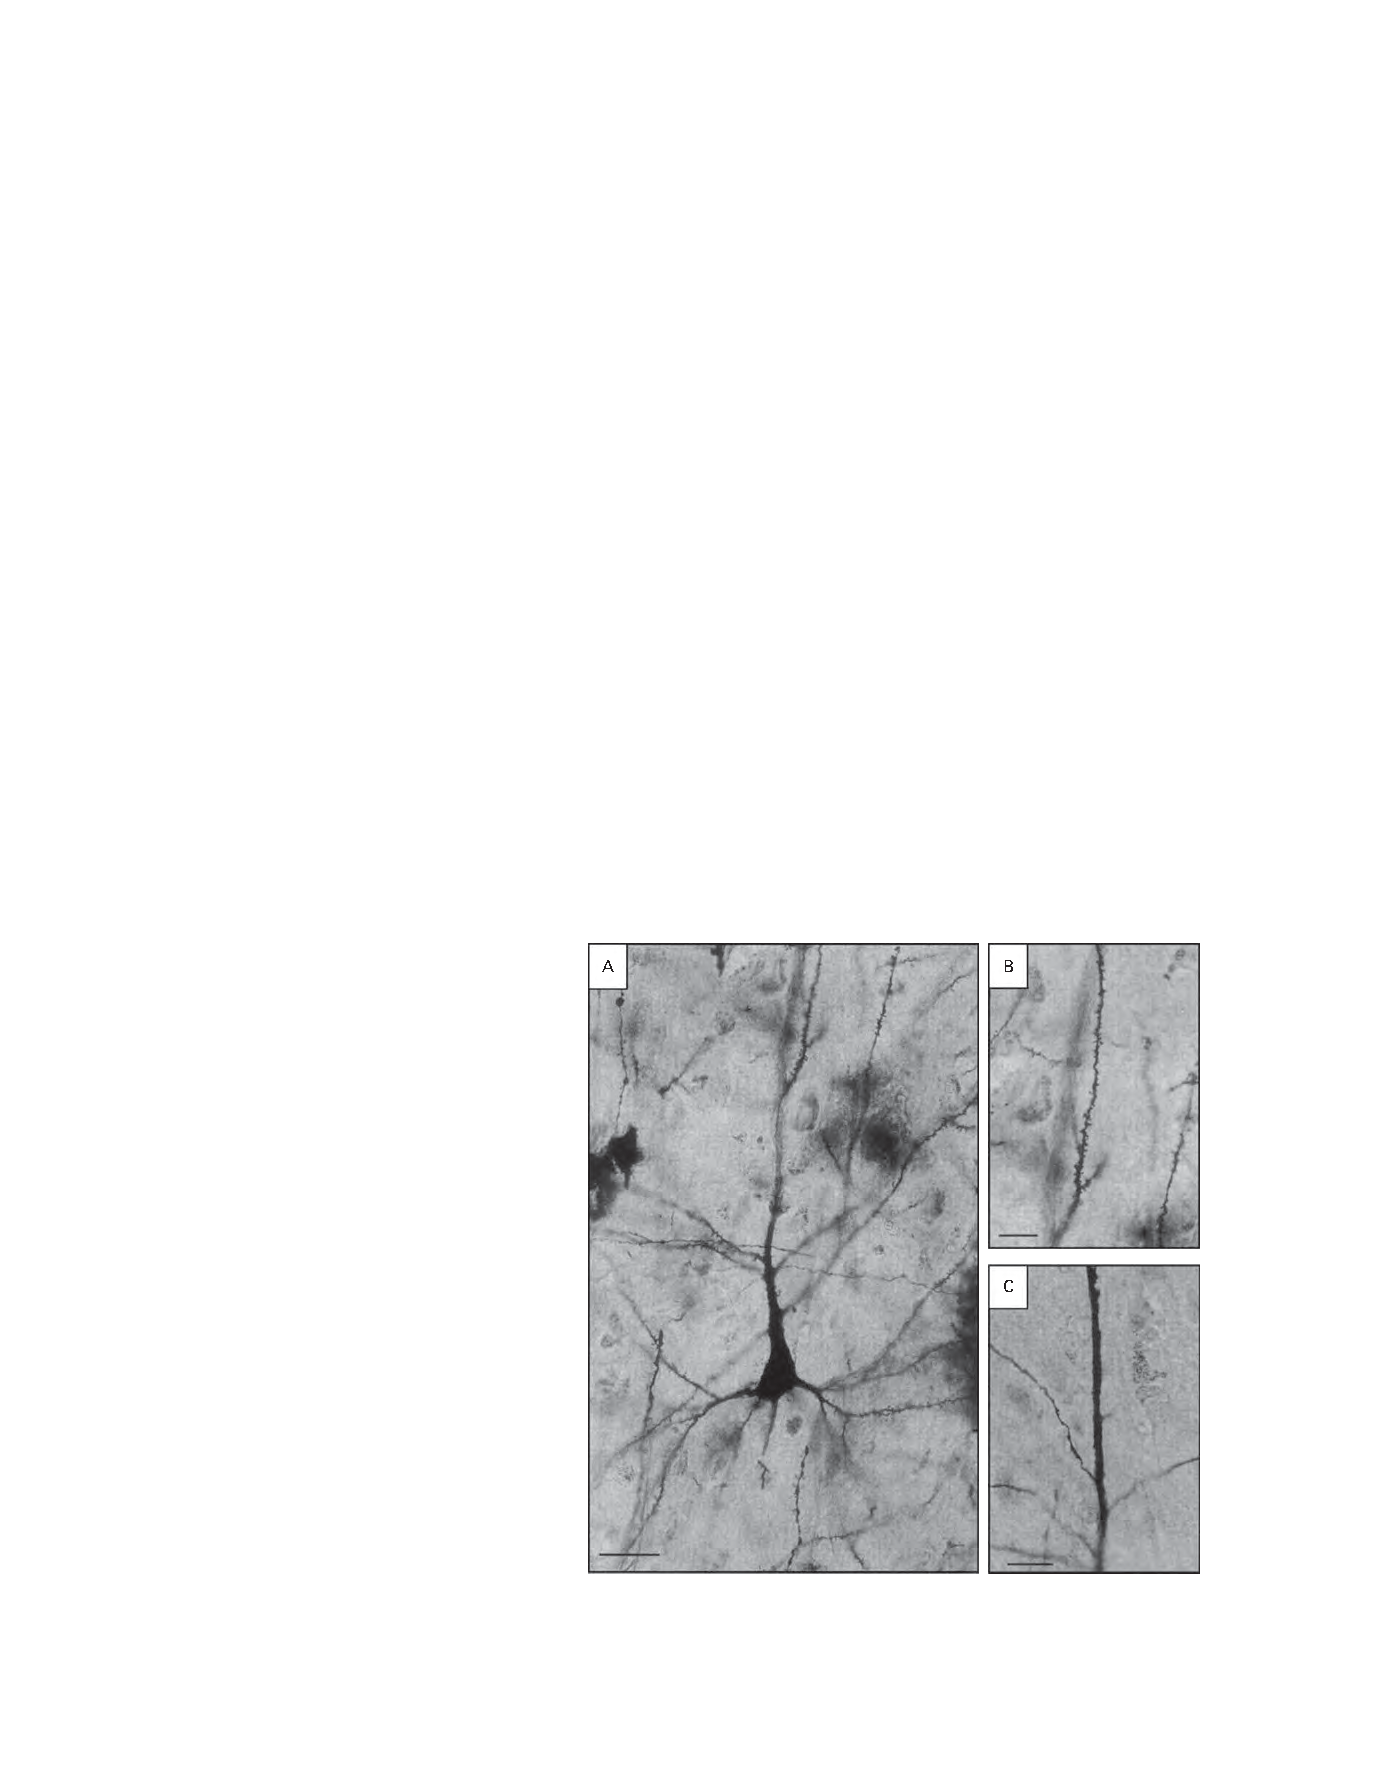
\includegraphics[width=0.7\linewidth]{chap60/fig_60_6}
	\caption{用高尔基体法染色的人脑大脑皮层锥体神经元的显微照片。 A. 来自对照大脑的第 III 层锥体神经元,显示其形态和布满刺的树突。 B. 更高倍视图显示控制大脑锥体神经元树突上的刺。 C. 精神分裂症患者大脑皮层的一段无刺的树突。 (比例:A:30 μm;B:20 μm;C:15 μm。)脊柱数粗略代表其他神经元与树突的突触接触数量; 因此,精神分裂症中棘突的缺乏与突触接触少于健康大脑大脑皮层中的突触接触是一致的。 (经许可转载,Garey 等人,1998 年。经 BMJ Publishing Group Ltd. 许可)}
	\label{fig:60_6}
\end{figure}

\subsection{青春期大脑发育异常可能导致精神分裂症}

精神分裂症在青春期晚期和成年早期之间表现出刻板印象,在精神病发作前数月或数年出现认知能力下降和阴性症状。 这个时间表明精神分裂症的发病机制可能涉及青春期大脑发育后期的异常,此时认知功能、情绪调节和执行功能通常成熟。

在整个发育过程中,神经元精心制作了大量的突触连接。 通常,突触在使用时会得到加强和保留,而弱或低效的突触会通过称为修剪的过程被消除。 涉及突触发生和修剪的突触细化过程导致高效且适应环境的神经计算。 依赖经验的突触细化首先在视觉皮层中被描述,其中弱连接的修剪对于双眼视觉的出现是必要的(见第 \ref{chap:chap49} 章)。 突触发生和修剪贯穿一生,使新的学习和旧记忆的更新成为可能。 然而,叠加在此类局部事件上的是显着的突触修剪浪潮,这些浪潮在空间上是特定的,在发育上是定时的。 人类大脑成熟的最后一波浪潮发生在青春期和成年早期,颞叶和前额叶联合皮层出现修剪。 这一后期修剪浪潮之后是这些皮层区域中许多轴突的髓鞘形成。

在 80 年代初期,欧文范伯格假设精神分裂症可能是由于青春期异常和过度的突触修剪所致。 随后对精神分裂症患者的大脑进行的尸检表明,前额叶和颞叶皮质的树突棘和突触减少。 对非人类灵长类动物的研究,以及人类尸检和神经影像学研究表明,树突状乔木的丧失并不是许多精神分裂症患者服用抗精神病药物的结果。 在此期间出现的认知障碍和负面症状与突触修剪不知何故失控、损害大脑皮层处理信息的能力的观点是一致的。 当过度修剪假说在 1980 年代首次提出时,它缺乏一个似是而非的分子或细胞机制来解释突触修剪如何在精神分裂症中出错。 最近的基因分析可能提供了一个解决方案。

无偏见的大规模遗传学研究发现,与精神分裂症风险的最强关联在于 6 号染色体上的主要组织相容性 (MHC) 基因座。MHC 基因座编码许多与免疫功能有关的蛋白质。 基因座的精细定位将最大的遗传关联信号精确定位到编码补体因子 C4 的基因,补体因子 C4 是经典补体级联的一个组成部分,在大脑外部参与标记微生物和受损细胞以供吞噬细胞吞噬和破坏。 随后的分析表明,随着 C4A(两种亚型之一)在大脑中表达的增加,精神分裂症的风险升高。 
这一发现增加了对过度修剪假说的支持,因为大脑中补体系统的一个功能是标记微弱或低效的突触以供小胶质细胞去除(图 \ref{fig:60_7})。

\begin{figure}[htbp]
	\centering
	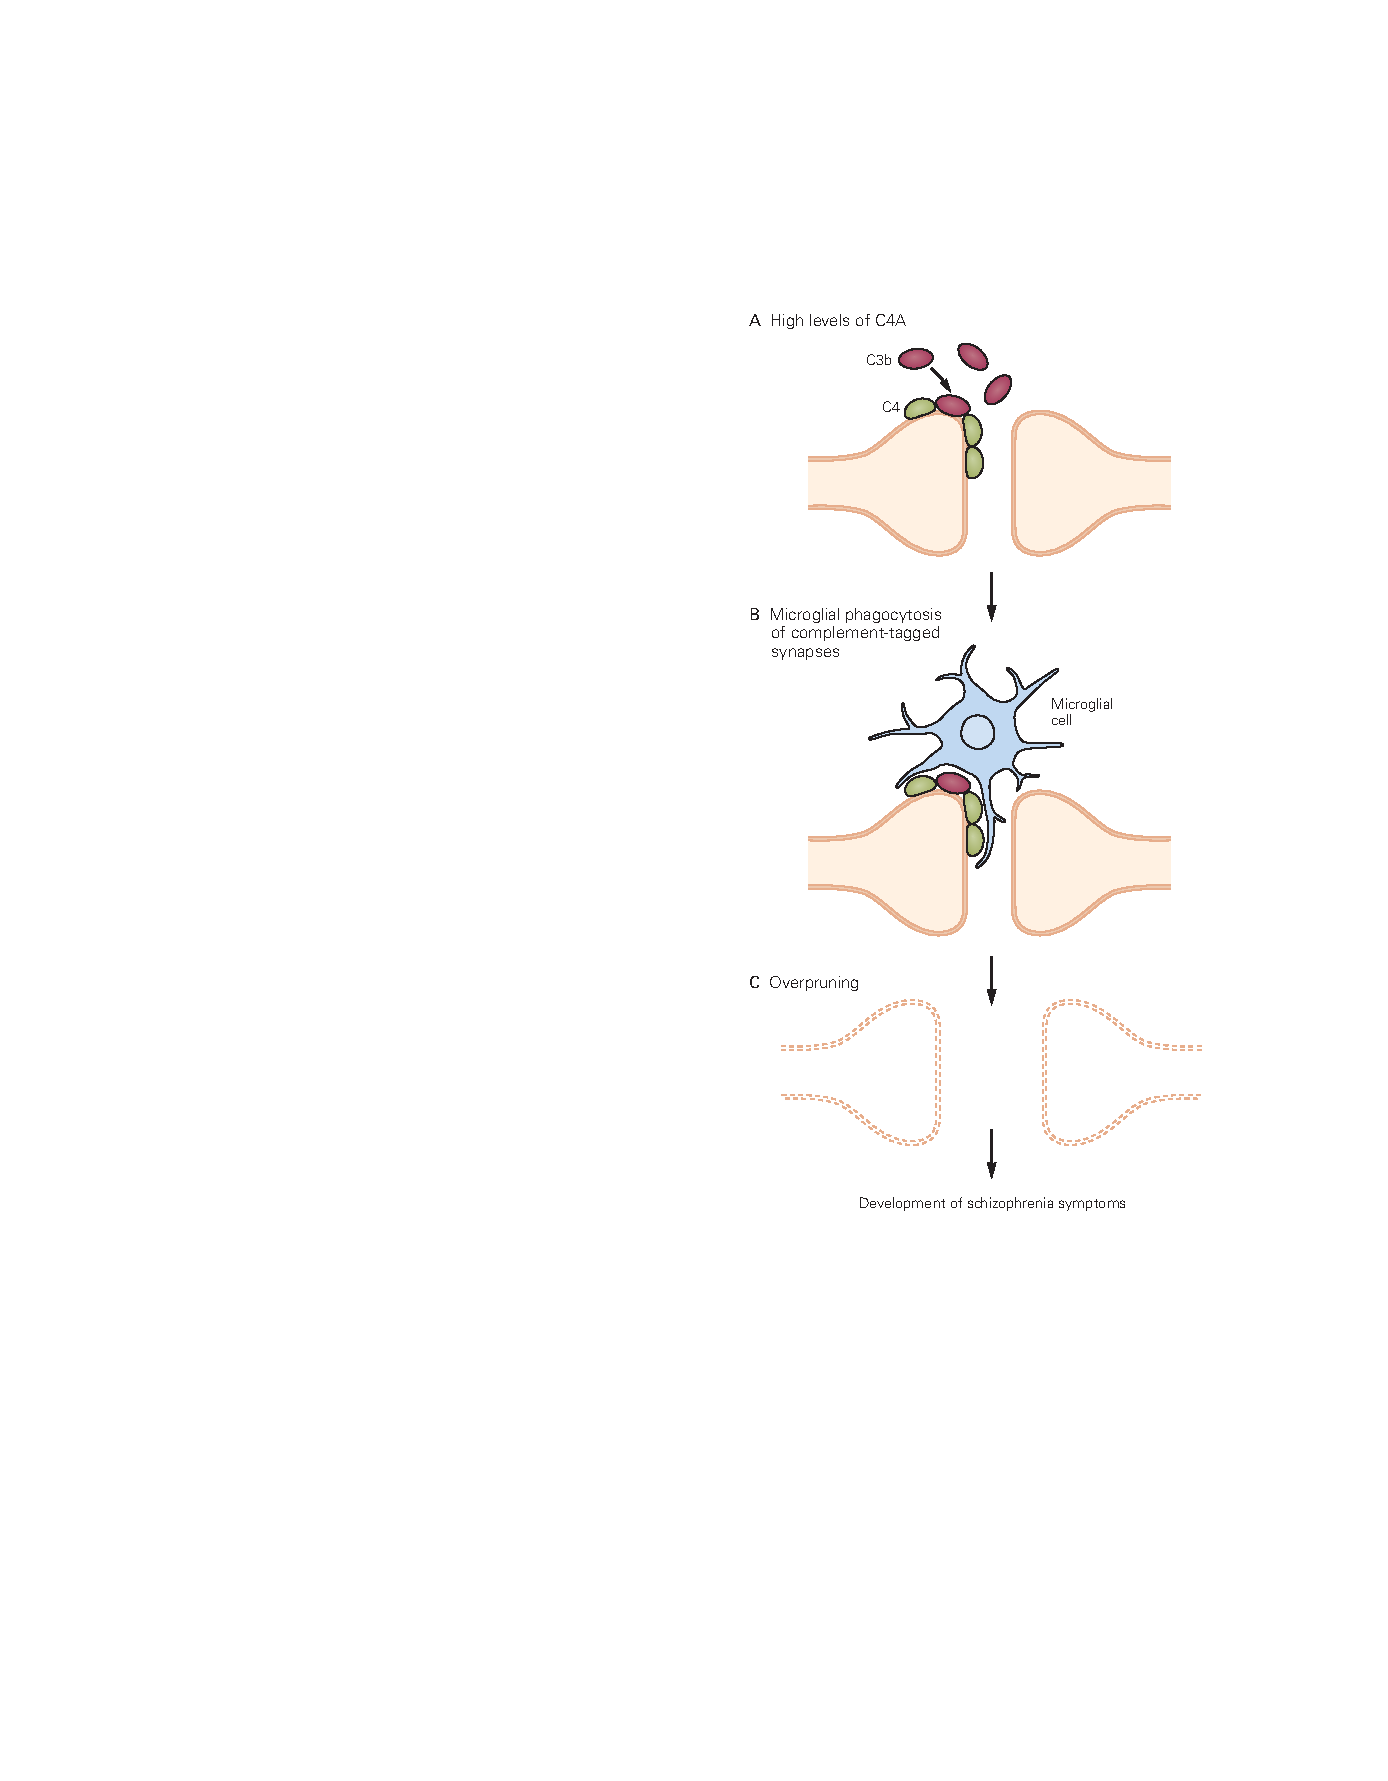
\includegraphics[width=0.45\linewidth]{chap60/fig_60_7}
	\caption{补体因子和小胶质细胞在突触消除中起作用。 神经系统的成熟和可塑性涉及突触发生和弱突触的消除。 补体因子 3b (C3b) 被认为是一种“惩罚信号”,可识别小胶质细胞吞噬作用的弱突触。 补体因子 4 (C4) 是补体级联的一个组成部分,由神经元和星形胶质细胞合成,并将 C3b 募集到弱突触。 在人类中,6 号染色体上的一个复杂基因组位点包含不同数量的基因拷贝,这些基因编码补体因子 C4 蛋白 C4A 和 C4B。 该基因座内的变异会导致大脑中 C4A 高水平表达,从而增加精神分裂症的风险。 (经许可转载自 Christina Usher 和 Beth Stevens。)}
	\label{fig:60_7}
\end{figure}

参与突触修剪的补体因子 C4A 的表达升高当然不是导致精神分裂症的唯一机制。 与任何多基因疾病一样,没有一个基因对于疾病表型是必要的或充分的。 因此,并非每个患有精神分裂症的人都具有高危 C4A 基因型,也并非每个具有高危 C4A 基因型的人都会发展为精神分裂症。 许多其他基因与精神分裂症的风险有关。 除了 C4 之外,还有一些这样的风险因素参与了补体级联的调节,但绝大多数都没有。 迄今为止已确定的许多与精神分裂症相关的基因都涉及突触结构和功能的各个方面; 几个编码离子通道。 因此,精神分裂症的遗传风险似乎至少部分涉及突触功能、突触可塑性和突触修剪,青春期突触过度修剪是一种似是而非的机制,应在高危青年研究中进一步探索 对于精神分裂症。 然而,其他尚未被充分表征的途径也可能被证明是重要的。 我们在理解精神分裂症的发病机制方面还有很长的路要走。

\section{抗精神病药物作用于大脑中的多巴胺能系统}
目前所有的抗精神病药物都是通过阻断前脑中的 D2 多巴胺受体来产生治疗效果的。 这些药物对各种神经递质受体和细胞内信号通路有许多其他作用,但这些其他作用主要影响它们的副作用,而不是它们的主要治疗机制(图 \ref{fig:60_8})。

\begin{figure}[htbp]
	\centering
	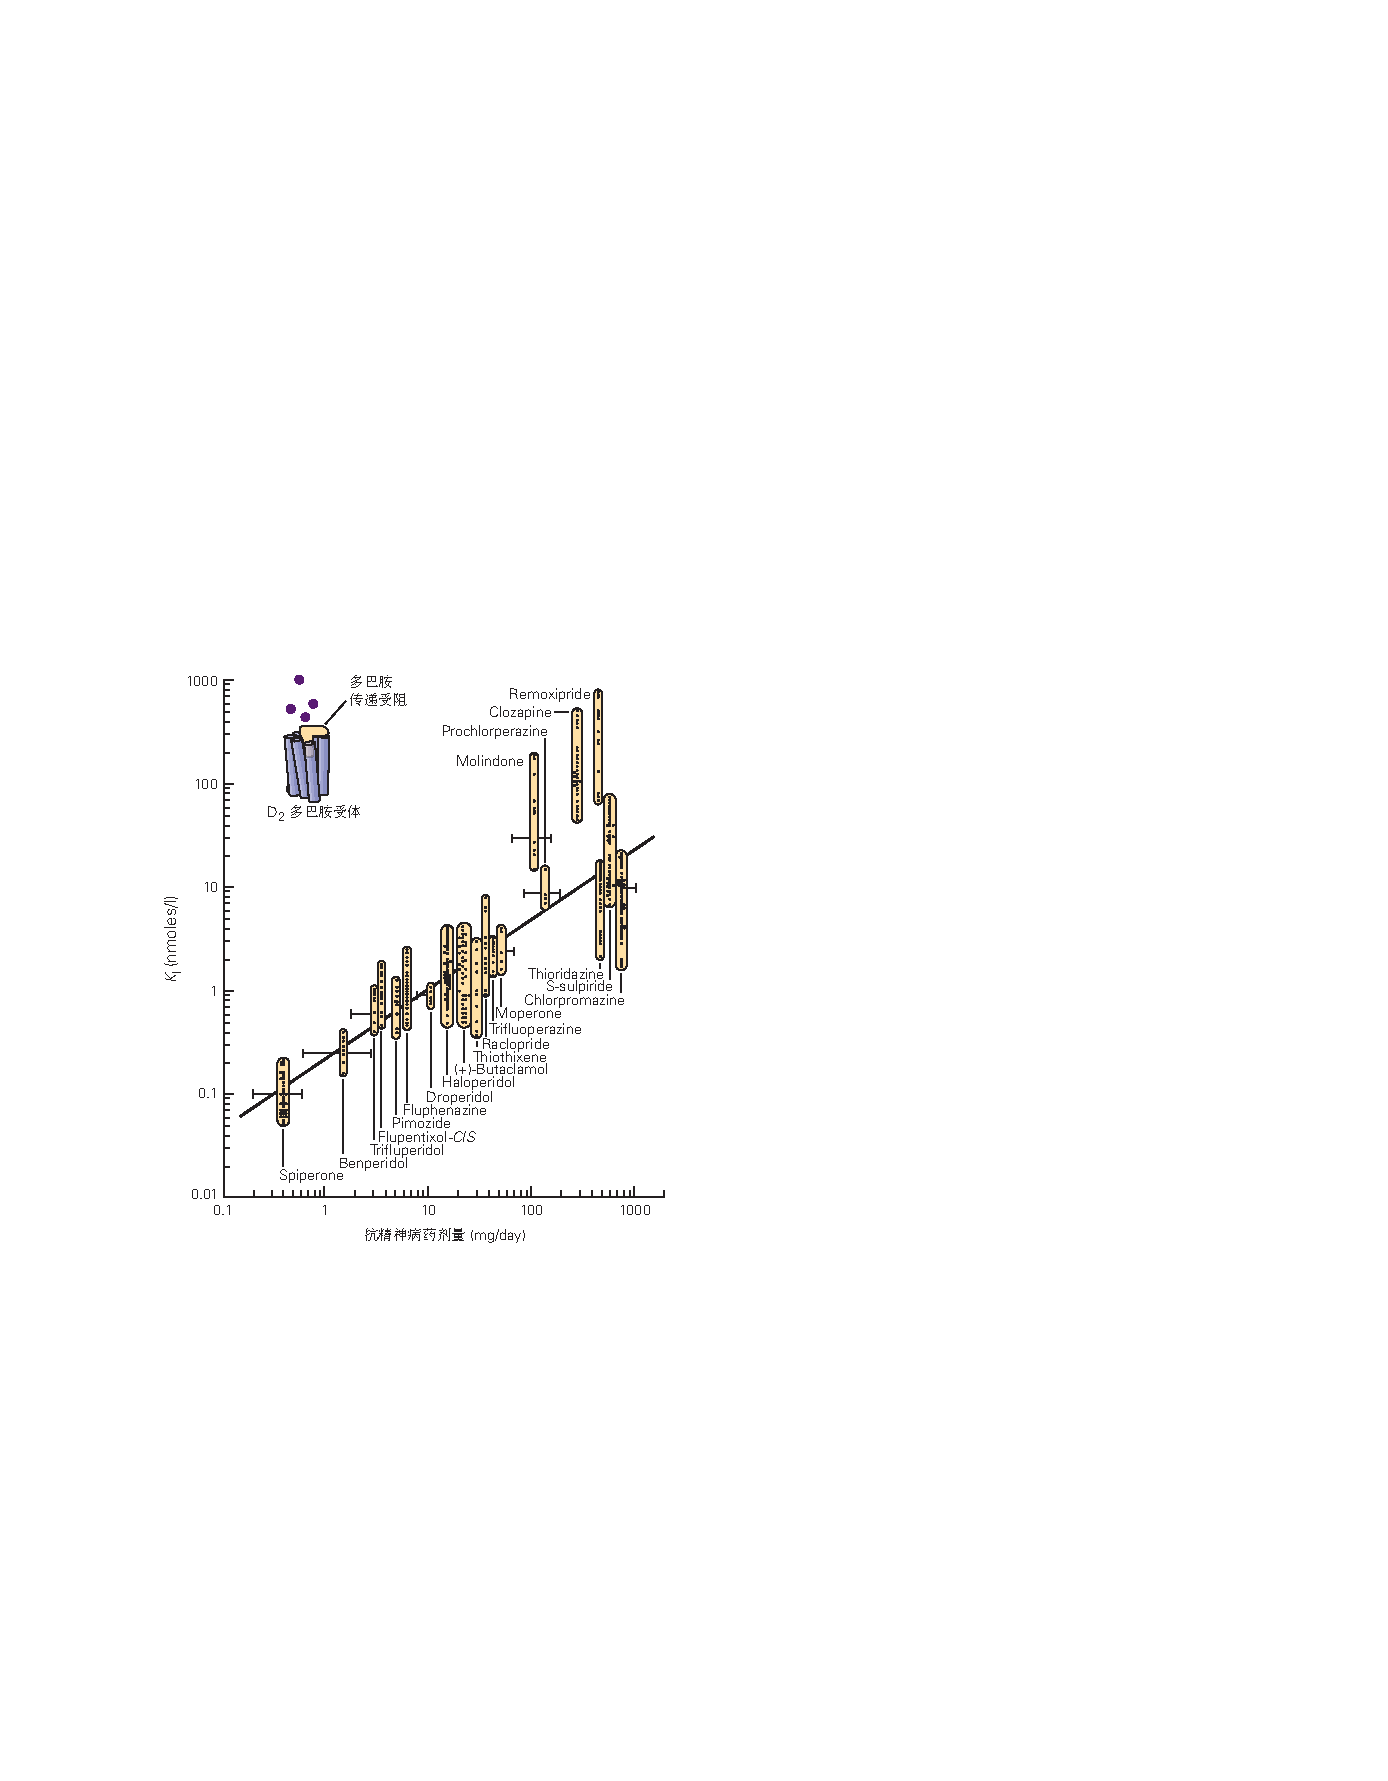
\includegraphics[width=0.5\linewidth]{chap60/fig_60_8}
	\caption{第一代抗精神病药物治疗精神病症状的效力与其对 D2 多巴胺受体的亲和力密切相关。 横轴是达到相似临床疗效水平所需的平均日剂量。 纵轴是 Ki,即体外结合 50\% D2 受体所需的药物浓度。 所需的药物浓度越高,药物对受体的亲和力就越低。 需要注意的是,两个轴上的测量值并不完全相互独立,因为药物在体外阻断 D2 受体的能力通常被用来帮助确定临床试验中使用的剂量。 不落下线的氯氮平,疗效明显优于其他。 其更大功效的机制尚不清楚。 (经许可改编自 Seeman 等人,1976 年。)}
	\label{fig:60_8}
\end{figure}

第一种有效的抗精神病药物氯丙嗪因其抗组胺和镇静作用而开发,并于 1952 年由 Henry Laborit 首次作为手术前麻醉剂进行研究。基于其镇静作用,此后不久就在精神病患者身上进行了测试。 令人惊讶的是,这些测试表明幻觉和妄想减少了; 事实上,氯丙嗪的镇静作用现在被认为是一种副作用。 氯丙嗪的成功促使人们尝试发现其他抗精神病药物。 尽管现在使用了许多化学性质不同的抗精神病药物,但它们都具有氯丙嗪在大脑中的相同初始作用,即阻断 D2 多巴胺受体的能力。 作为一类药物,这些药物不仅可以改善精神分裂症的精神病症状,还可以改善双相情感障碍、严重抑郁症和各种神经退行性疾病的精神病症状。 没有一种抗精神病药物能有效治疗精神分裂症的认知障碍或缺陷症状。

在它们的副作用中,氯丙嗪和相关药物会引起帕金森样运动症状。 由于帕金森病是由中脑中多巴胺能神经元的丢失引起的,因此帕金森样副作用的发生向 Arvid Carlsson 表明这些药物通过减少多巴胺能传递起作用。 按照这个想法,卡尔森确定抗精神病药物会阻断多巴胺受体。 已知有两个多巴胺受体家族。 D1 家族(在人类中包括 D1 和 D5)与激活腺苷酸环化酶的刺激性 G 蛋白偶联。 D2 家族,包括 D2、D3 和 D4,与抑制环化酶并激活超极化 K+ 通道的抑制性 G 蛋白 (Gi) 偶联。 D2 受体的第二条信号通路由 β-arrestin 介导。 D1 受体在纹状体中表达,是大脑皮层和海马体中的主要一类多巴胺受体。 D2受体在纹状体、大脑皮层、杏仁核和海马体中表达最密集。 受体结合研究与精神病症状临床疗效之间的相关性表明 D2 家族是抗精神病药物治疗作用的分子靶标。

氯氮平是 1959 年发现的一种抗精神病药物,引起帕金森样运动副作用的可能性很低。 然而,由于它有一些严重的副作用,包括可能导致血液粒细胞致命损失的可能性很小,因此停止使用,直到 80 年代后期的一项临床试验清楚地表明它比其他抗精神病药物具有更大的疗效。 氯氮平改善了一些对其他抗精神病药物没有反应的个体。 它与每周监测白细胞计数一起重新引入; 试图与氯氮平媲美的尝试也推动了第二代抗精神病药物的开发,该药物模仿其某些受体结合特性,特别是阻断 5-羟色胺 5-HT2A 受体的能力,这种作用似乎可以减少运动副作用。 第二代抗精神病药物的大规模临床试验表明,其疗效不大于第一代药物,没有与氯氮平相当的疗效。 第二代药物引起帕金森样运动副作用的可能性低于第一代,但它们通常会导致更严重的体重增加和其他代谢问题。

由于药物通过阻断 D2 受体来减轻精神病症状,因此研究人员提出疑问:多巴胺在精神分裂症症状中的作用是什么? 虽然一些阻断 D2 受体的药物可以减轻精神病症状,但其他增加突触多巴胺的药物,如苯丙胺和可卡因,在长期大剂量服用时会产生精神病症状。 因此,Carlsson 认为多巴胺能系统在精神分裂症中过度活跃。 这一假设的证据很难获得。 支持这一想法的最直接证据来自于 20 世纪 90 年代中期开始的研究,这些研究发现精神分裂症患者中安非他明引起的多巴胺释放增加比健康受试者更大。 这些研 对抗精神病药物有反应。

尽管精神分裂症大脑皮层下区域的多巴胺活性可能增加,但在皮层区域可能会减少; 这种减少可能会导致精神分裂症中出现的认知障碍。 特别是,精神分裂症患者前额皮质中的 D1 受体可能较少,这与前额皮质中的 D1 受体通常在工作记忆和执行功能中发挥作用的观察结果一致。


\section{亮点}

1. 精神分裂症是一种慢性、严重致残的疾病,其特征是剧烈的精神病症状以及情绪、动机和认知缺陷。 

2. 精神分裂症的风险是一种遗传性多基因特征。 

3. 抗精神病药物可有效减少幻觉、妄想和思维障碍,但对精神分裂症的认知和缺陷症状无益。 

4. 认知障碍降低了精神分裂症患者根据自己的目标调节行为的能力。 因此,精神分裂症患者常常无法在学业上取得成功或保住工作,即使在抗精神病药物有效控制幻觉和妄想的情况下也是如此。 

5. 尸检和神经影像学研究记录了前额叶和颞叶大脑皮层中灰质的丢失,其模式与认知障碍一致,例如工作记忆缺陷。 

6. 灰质损失是由树突分枝减少和树突棘减少引起的,这意味着突触连接也减少了。 与这些解剖学发现和典型的青春期发病年龄一致的假设是,精神分裂症是由青春期和成年早期前额叶和颞叶大脑皮层过度和不适当的突触修剪引发的。 

7. 精神分裂症基因分析的进展结合使用新工具研究系统级神经科学有望帮助在理解疾病机制和发现新疗法方面取得急需的进展。


%\subsection{选读}
%\subsection{参考文献}
